\chapter[Resultados]{Resultados}

Este capítulo irá apresentar os resultados obtidos durante a realização deste trabalho. Serão mostrados os prótotipos iniciais do jogo, a \textit{engine} desenvolvida para a construção do jogo e, por fim, as telas do jogo final desenvolvido.

\section{Protótipo inicial}

A fim de atestar a viabilidade do porte do jogo \textit{Traveling Will}, desenvolvido inicialmente para PC, para a plataforma \textit{Nintendo Game Boy Advance}, foi feita uma versão funcional do menu original do jogo, já testada em um \textit{Nintendo DS} (como explicado na Seção \ref{console} do Capítulo \ref{metodologia}). Para isso, a principal ferramenta utilizada foi a \textit{libtonc}\footnote{\textit{libtonc}, disponível em \url{http://www.coranac.com/files/tonc-code.zip}}, que nessa versão inicial fez o papel de \textit{engine} do jogo.

Abaixo é possível comparar o menu principal do jogo original com o protótipo implementado sendo executado em um emulador de \textit{Game Boy Advance}:

\begin{figure}[H]
 \centering \includegraphics[keepaspectratio=true,scale=0.6]{figuras/tw-original-1.eps}
   \caption[Jogo original sendo executado em um PC]
    {Jogo original sendo executado em um PC. Fonte: \textit{Autores}.}
   \label{tw-original-1}
\end{figure}

\begin{figure}[H]
 \centering 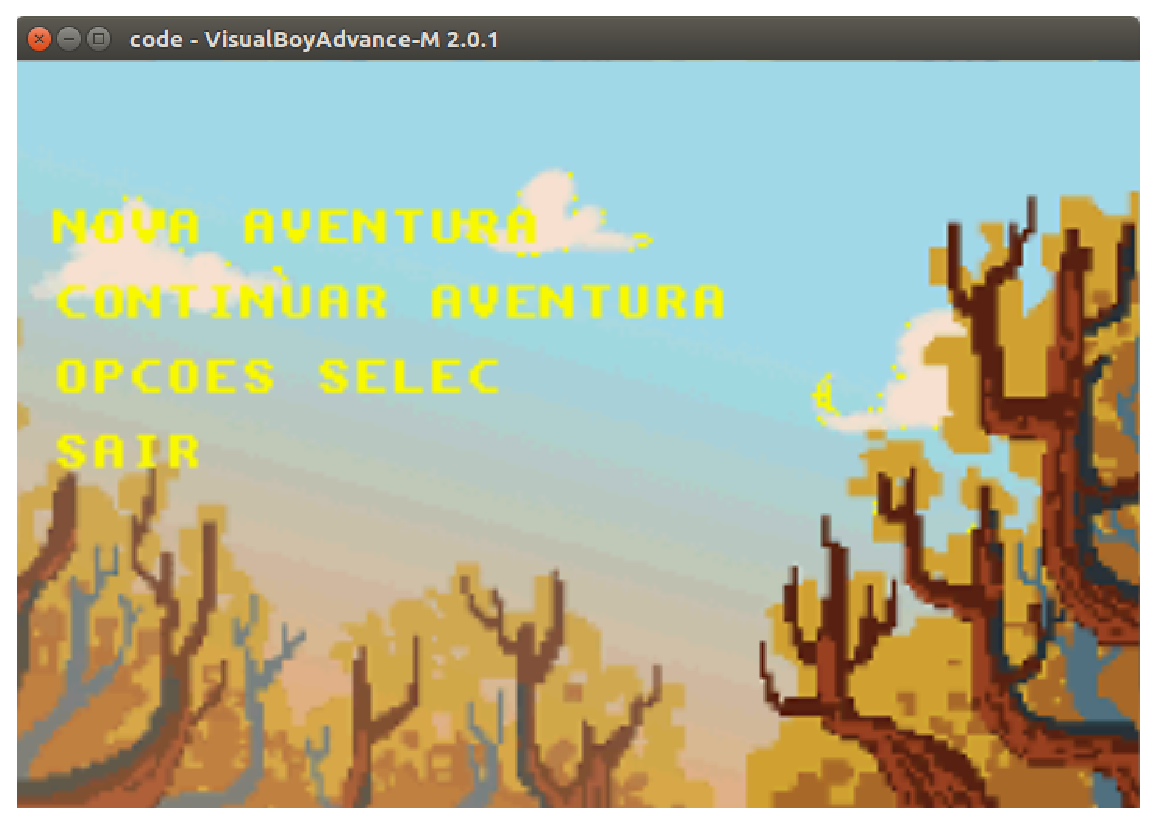
\includegraphics[keepaspectratio=true,scale=0.6]{figuras/tw-gba-1.eps}
   \caption[Protótipo sendo executado no emulador de GBA]
    {Protótipo sendo executado no emulador de GBA. Fonte: \textit{Autores}.}
   \label{tw-gba-1}
\end{figure}

Este protótipo inicial contém apenas a tela vista acima, com um \textit{background} desenhado ao fundo e quatro botões clicáveis, porém sem nenhuma ação após o clique. Para alterar o botão selecionado, basta

O protótipo desenvolvido está disponível no seguinte repositório: \url{https://github.com/traveling-will-gba/traveling-will-prototype}

\section{Desenvolvimento da \textit{engine}}

Logo após a finalização do protótipo, foi iniciado o desenvolvimento da \textit{engine} responsável por substituir a \textit{libtonc} e gerenciar os recursos do jogo. Esta \textit{engine} contém os seguintes módulos: \textit{input}, vídeo, gerenciador de memória, áudio e física. Além disso, a \textit{engine} contém abstrações para os níveis (\textit{levels}) e objetos do jogo (\textit{game objects}) e um módulo utilitário para funções genéricas relacionadas ao \textit{hardware} do GBA.

Os módulos de vídeo, \textit{input}, física e as abstrações para níveis e objetos do jogo foram desenvolvidos tendo como base a \textit{ijengine}\footnote{\textit{ijengine}, disponível em \url{https://github.com/fgagamedev/ijengine}}, \textit{engine} desenvolvida para a disciplina de Introdução aos Jogos Eletrônicos, que tem como foco a criação de jogos para PC utilizando \textit{C++}. Ela contém módulos de vídeo, áudio, manipulação de eventos, física, \textit{input}, dentre outros, e contém uma interface para a utilização de diferentes bibliotecas gráficas, como SDL\footnote{\textit{Simple DirectMedia Layer}, disponível em \url{https://www.libsdl.org}} e OpenGL\footnote{OpenGL, disponível em \url{https://www.opengl.org}}.

\subsection{Módulo de \textit{input}}

Os estados dos botões do GBA ficam salvos em um registrador. Cada um desses estados é representado por um \textit{bit} do valor guardado por esse registrador. Sempre que um botão é pressionado, o GBA automaticamente troca o valor guardado nesse registrador de tal forma que o \textit{bit} que representa o botão em questão passe a possuir valor 0. De forma similar, quando o botão é solto, o valor contido no \textit{bit} em questão é modificado para 1, seu valor padrão. Sendo assim, a checagem dos estados pode ser realizada facilmente utilizando \textit{bitmasks}.

Por exemplo, caso se deseje checar um botão representado pelo \textit{bit} 2 (com a contagem começando em 0), basta pegar o resultado do \textit{AND} binário entre o valor guardado no registrador e a potência de 2 que possui como expoente o \textit{bit} em questão (4, nesse exemplo). No Código \ref{lst:input1} é possível visualizar a definição das constantes que representam os botões. A função utilizada para checar o estado de cada um deles pode ser vista no código \ref{lst:lalala}.

\begin{lstlisting}[caption={Cabeçalho do módulo de \textit{input}.},label={lst:input1}]
#ifndef INPUT_H
#define INPUT_H

#include <stdbool.h>
#include "base_types.h"

#define BUTTON_A 1
#define BUTTON_B 2
#define BUTTON_SELECT 4
#define BUTTON_START 8
#define BUTTON_RIGHT 16
#define BUTTON_LEFT 32
#define BUTTON_UP 64
#define BUTTON_DOWN 128
#define BUTTON_R 256
#define BUTTON_L 512
#define N_BUTTON 10

int pressed_state[N_BUTTON];

void check_buttons_states();
bool pressed(int button);

#endif
\end{lstlisting}

\begin{lstlisting}[caption={Código-fonte do módulo de \textit{input}.},label={lst:lalala}]
int pressed_state[N_BUTTON];
uint64_t key_update[N_BUTTON];
uint64_t update_counter;

void check_buttons_states() {
    update_counter++;

	for(int i = 0; i < N_BUTTON; i++) {
        int pressed = !((*buttons_mem) & (1 << i));

        if (pressed == pressed_state[i]) continue;

        pressed_state[i] = pressed;
        key_update[i] = update_counter;
	}
}

bool pressed(int button) {
	return pressed_state[32 - __builtin_clz(button) - 1] && key_update[32 - __builtin_clz(button) - 1] == update_counter;
}

bool pressing(int button) {
	return pressed_state[32 - __builtin_clz(button) - 1];
}
\end{lstlisting}

A Figura \ref{demo-input} apresenta o teste implementado para checar o pressionamento dos botões do GBA. Para cada botão pressionado um \textit{pixel} vermelho aparece na tela. Nesta figura, os botões B, R, \textit{LEFT}, \textit{DOWN} e \textit{START} estão sendo pressionados simultaneamente. O código \ref{lst:inputtest} apresenta este teste.

\begin{figure}[H]
 \centering 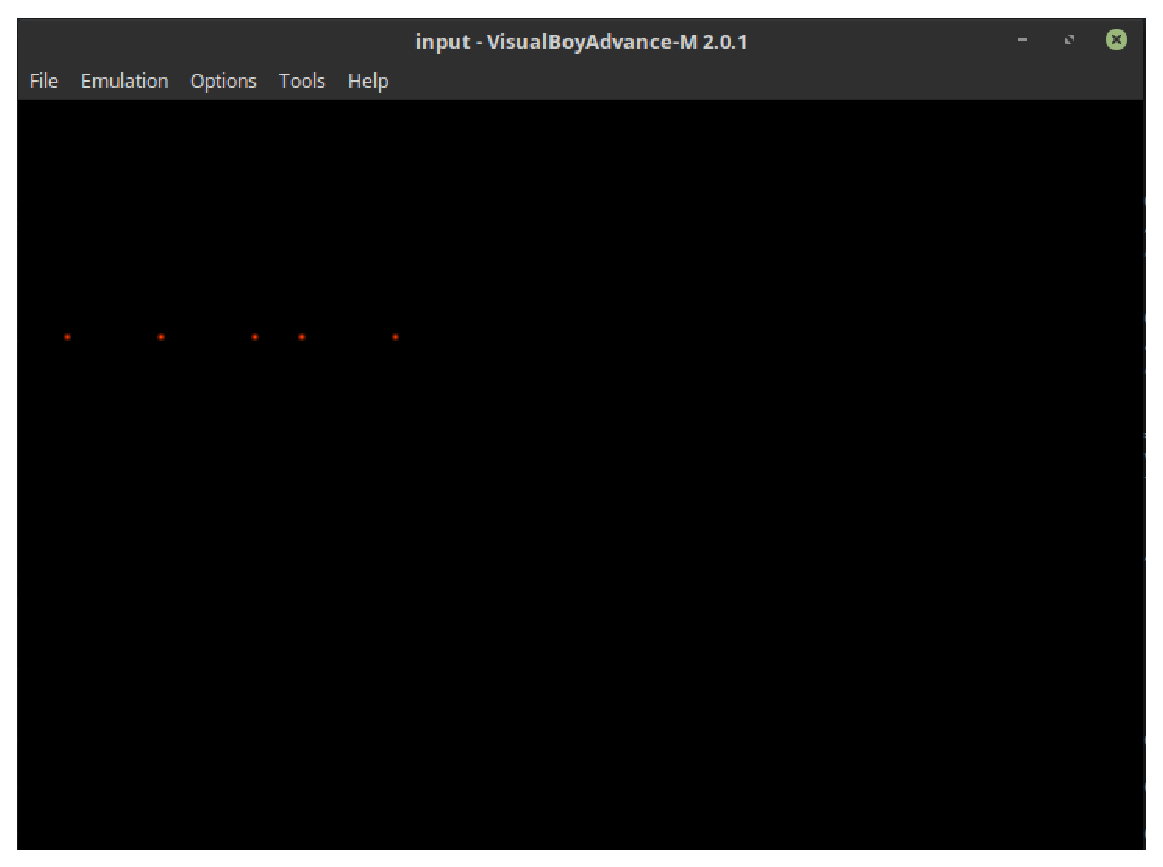
\includegraphics[keepaspectratio=true,scale=0.6]{figuras/demo-input.eps}
   \caption[Demonstração do pressionamento de botões no emulador]
    {Teste de pressionamento de botões no emulador.}
   \label{demo-input}
\end{figure}

\begin{lstlisting}[float,caption={Código de teste de \textit{input}.},label={lst:inputtest}]
#include "video.h"
#include "input.h"
#include "utils.h"

#define RED 0x0000FF

volatile unsigned short *vid_mem = (unsigned short *)0x6000000;

int main() {
	reset_dispcnt();
	set_video_mode(3);
	enable_background(2);

    while(1) {
        check_buttons_states();

        for(int i=0;i<=9;i++){
            int padding = i + 10;

            if (pressing(1 << i)) {
                for(int x=-2;x<=2;x++) {
                    for(int y=-2;y<=2;y++) {
                        vid_mem[(50 + x) * 240 + (20 + y + i * 10)] = RED;
                    }
                }
            }
            else {
                for(int x=-2;x<=2;x++) {
                    for(int y=-2;y<=2;y++) {
                        vid_mem[(50 + x) * 240 + (20 + y + i * 10)] = 0;
                    }
                }
            }
        }
    }

    return 0;
}
\end{lstlisting}

O código deste projeto se encontra no seguinte endereço: \url{https://bit.ly/2BQV6jf}.

\subsection{Módulo gerenciador de memória}

Para melhor utilização dos recursos providos pelo GBA foi desenvolvido um módulo que trata do gerenciamento de memória dos objetos do jogo. A principal responsabilidade deste módulo é garantir que a alocação e desalocação de recursos seja feita de forma eficiente e segura.

    \subsubsection{Funcionamento do gerenciador de memória}

    O modelo de gerenciamento escolhido para ser utilizado neste projeto foi o modelo de gerenciamento com partições variáveis \cite{tanenbaum}. Esse modelo se faz necessário pois os recursos a serem alocados durante a execução do jogo contém tamanhos distintos (uma sprite ocupa menos espaço que um \textit{background} que, por sua vez, ocupa menos espaço do que uma música). Além disso, é importante citar que este gerenciador aloca os recursos contiguamente na memória, isto é, ele sempre irá optar pelo primeiro espaço disponível a partir do começo da memória.

    Utilizando esse modelo como base, o gerenciador funciona da seguinte maneira:

    \begin{itemize}
        \item o construtor do gerenciador de memória é responsável por inicializar todos os ponteiros correspondentes aos endereços dos registradores de \textit{backgrounds}, texturas e atributos das texturas;
        \item quando ocorre uma chamada de alocação, o gerenciador procura pelo primeiro espaço disponível na memória correspondente para alocar tal recurso. Caso não ache nenhum espaço disponível, retorna um endereço nulo;
        \item após achar um endereço disponível, é verificado se há espaço suficiente para alocar o recurso. Caso não haja espaço suficiente, um endereço nulo é retornado;
        \item após garantir que há um espaço disponível e com espaço suficiente para alocação, a posição deste endereço no vetor auxiliar (responsável por indicar se determinado endereço está disponível ou não) é ligada (indicando que o espaço foi ocupado) e é retornado o endereço desta posição para o cliente (no caso, o jogo) realizar a cópia do recurso.
    \end{itemize}

    O código \ref{lst:alloc} apresenta a função responsável por realizar a alocação de paletas (tanto para \textit{backgrounds} quanto para texturas). Segundo \citeonline{gbatek}, as paletas possuem 256 entradas de 2 \textit{bytes}, totalizando 512 \textit{bytes}.

    \begin{lstlisting}[float,caption={Código de alocação de paletas para \textit{backgrounds} e texturas.},label={lst:alloc}]
    volatile uint8_t *MemoryManager::alloc_palette(bitset<512>& used,
        volatile uint8_t *palette, size_t size)
    {
        int used_size = used.size();

        for (size_t i = 0; i < used_size; i++) {
            // if this position is taken, skip it
            if (used[i] == true) {
                continue;
            }

            uint32_t available_pal_len = used_size - i;

            // if there is no space to allocate this pallete, skip it
            if (size > available_pal_len) {
                continue;
            }

            // mark positions from i to size as used
            for (size_t j = 0; j < size; j++) {
                used[i + j] = true;
            }

            memory_map[palette + i] = size;

            return palette + i;
        }

        return NULL;
    }
    \end{lstlisting}


    \subsubsection{Gerenciamento de memória}

    Para garantir que novos recursos sejam alocados e que nenhum objeto já carregado na memória seja sobrescrito ou corrompido, qualquer chamada que envolva a alocação de novos recursos passa por um processo onde é verificado se a memória que será populada contém espaço suficiente realizar tal alocação.

    Para realizar esta verificação, o gerenciador possui um mapa que associa um endereço na memória com o tamanho que o objeto alocado neste endereço ocupa. Deste modo, quando há uma chamada de alocação com tamanho \texttt{size} e uma posição \texttt{i} está disponível e o tamanho da partição em \textit{bytes} é dado por \texttt{t}, as posições de \texttt{i} até $ i + \frac{size}{t} - 1 $ são marcadas como utilizadas.

    As estratégias utilizadas para garantir um gerenciamento eficiente de memória envolvem a utilização de \textit{singleton} para a criação do objeto gerenciador de memória e utilização de estruturas de dados que permitam configurar o tamanho a ser utilizado.

    Para que haja um único objeto encarregado de gerenciar a alocação de recursos no jogo, a classe \texttt{MemoryManager} foi modelada utilizado o padrão de projeto \textit{Singleton}. Com este padrão de projeto, cada chamada de criação de uma nova instância do gerenciador de memória passa por uma verificação, que checa se já existe uma instância desta classe (por meio de uma variável dentro da própria classe que armazena uma instância de \texttt{MemoryManager} ou nulo). Caso haja, esta instância é retornada. Caso contrário, é criada uma nova instância. O código \ref{lst:manager} exemplifica o \textit{singleton} (trechos de código desta classe foram omitidos para melhor foco no padrão de projeto):

\begin{lstlisting}[caption={\textit{Singleton} do gerenciador de memória.},label={lst:manager}]
class MemoryManager {
    private:
        MemoryManager *instance;
    public:
        MemoryManager *get_memory_manager() {
            if (!instance) {
                instance = new MemoryManager();
            }
            return instance;
        }
};
\end{lstlisting}

A fim de não utilizar memória desnecessariamente, em alguns pontos do jogo foram utilizadas estruturas que permitem configurar a quantidade de \textit{bits} que podem ser utilizados por cada variável. O primeiro exemplo mostra uma \texttt{struct} que armazena os atributos das texturas, onde cada atributo só precisa de um pequeno número de \textit{bytes}. Já o segundo exemplo demonstra a utilização de \texttt{bitsets} (que mantém a disponibilidade de cada posição do endereço de memória) com tamanho fixo correspondente ao tamanho total da respectiva região de memória (neste exemplo, \texttt{Video RAM}).

\begin{lstlisting}[float,caption={\texttt{Struct} com \texttt{bitfields} para atributos das texturas.}]
struct attr {
    // attr0
    uint8_t y;
    uint8_t om : 2;
    uint8_t gm : 2;
    uint8_t mos : 1;
    uint8_t cm : 1;
    uint8_t sh : 2;
    // attr1
    uint16_t x : 9;
    uint8_t aid : 5;
    uint8_t sz : 2;
    // attr2
    uint16_t tid : 10;
    uint8_t pr : 2;
    uint8_t pb : 4;
    // attr3
    uint16_t filler;
};
\end{lstlisting}

\begin{lstlisting}[float,caption={\textit{Bitsets} para checagem de disponibilidade na memória.}]
// backgrounds and textures have 512 bytes each for palette memory
bitset<512> background_palette_used;
bitset<512> texture_palette_used;
// max number of charblocks that can be stored in VRAM
bitset<4> charblock_used;
// max number of screenblocks that can be stored in VRAM
bitset<32> screenblock_used;
\end{lstlisting}


\subsection{Módulo de vídeo}

O módulo de vídeo é responsável pelo controle do modo de vídeo, dos \textit{backgrounds} e da renderização das \textit{sprites}.

Para gerenciar a renderização das \textit{sprites} foi desenvolvida uma classe chamada \textit{Texture}. Ela foi planejada de forma a não apenas copiar os dados da imagem para a região de memória apropriada, mas também permitir a animação das \textit{sprites} de uma textura e controlar os metadados das imagens renderizadas no jogo.

A seguir, será explicado, com o auxílo de trechos do código, o funcionamento dos principais elementos dessa classe.

Inicialmente, é necessário explicar os construtores dessa classe.

Logo abaixo, é possível visualizar o código do primeiro construtor. Ele recebe os ponteiros para a paleta de cores e para o vetor de \textit{tiles} utilizados pela imagem, os tamanhos das regiões de memória alocadas pra cada um desses ponteiros e a quantidade de \textit{bits} por \textit{pixel} que a imagem utiliza. Cada um desses atributos é guardado na própria classe, e, já nesse construtor, são chamados os métodos \textit{set\_sprite\_pal} e \textit{set\_sprite}, responsáveis por copiá-los para as regiões apropriadas. Por fim, ainda nesse construtor, são setados os índices do \textit{tile base} e da paleta de cores utilizada pela imagem. O cálculo desses índices será explicado logo adiante, nos tópicos dedicados aos métodos \textit{set\_sprite\_pal} e \textit{set\_sprite}.

\begin{lstlisting}[caption={Construtor da classe \textit{Texture}.}]
Texture::Texture(uint32_t num_sprites, const uint16_t *pallete, uint32_t pallete_len,
    const unsigned int *tiles, uint32_t tiles_len, enum bits_per_pixel bpp = _8BPP)
{
    this->pallete = pallete;
    this->pallete_len = pallete_len;
    this->pallete_id = 0;
    this->bpp = bpp;
    this->num_sprites = num_sprites;
    this->num_tiles = tiles_len / ((bpp == _4BPP) ? 32 : 64);
    this->tiles_per_sprite = num_tiles / num_sprites;
    this->tiles = tiles;
    this->tiles_len = tiles_len;

    memory_manager = MemoryManager::get_memory_manager();

    set_sprite_pal();
    set_sprite();
    oam_entry = memory_manager->alloc_oam_entry();

    metadata.tid = tile_base * ((bpp == _4BPP) ? 1 : 2);
    metadata.pb = pallete_id;
}
\end{lstlisting}
\vspace{\onelineskip}

O segundo construtor funciona de forma similar ao anterior, com a diferença de que em vez de receber todos os atributos da imagem, ele recebe apenas um ponteiro para outra textura. Esse construtor serve para quando se deseja renderizar réplicas de uma mesma textura. Utilizar ele permite que tais texturas compartilhem a paleta de cores e o vetor de \textit{tiles}, fazendo-se necessário alocar espaço apenas para os metadados, que são diferentes pra cada textura.

\begin{lstlisting}[caption={Construtor por cópia da classe \textit{Texture}.}]
Texture::Texture(const Texture *texture)
{
    this->num_sprites = texture->num_sprites;
    this->pallete = texture->pallete;
    this->pallete_len = texture->pallete_len;
    this->tiles = texture->tiles;
    this->tiles_len = texture->tiles_len;
    this->bpp = texture->bpp;
    this->pallete_id = texture->pallete_id;
    this->num_tiles = texture->num_tiles;
    this->tiles_per_sprite = texture->tiles_per_sprite;
    this->tile_base = texture->tile_base;

    memory_manager = MemoryManager::get_memory_manager();

    oam_entry = memory_manager->alloc_oam_entry();

    metadata.tid = tile_base * ((bpp == _4BPP) ? 1 : 2);
    metadata.pb = pallete_id;
}
\end{lstlisting}
\vspace{\onelineskip}

O método \textit{set\_sprite\_pal} é responsável por chamar o método \textit{alloc\_texture\_pal} da classe \textit{MemoryManager} passando como parâmetro o tamanho da paleta de cores a ser alocada. Como resultado, ele irá receber o endereço de memória aonde a paleta deverá ser guardada. Após fazer a cópia da paleta, é preciso calcular o índice da paleta escolhida na memória, já que esse é um dos metadados necessários para renderização da imagem a 4 \textit{bits} por \textit{pixel}. Como a região reservada para as paletas de cores no \textit{GBA} é divida em regiões de 32 \textit{bytes}, para realizar tal cálculo basta pegar a diferença entre o início da região escolhida para a cópia e o início da região reservada para as paletas e dividir por 32.
Como uma imagem renderizada a 8 \textit{bits} por \textit{pixel} ocupa toda a região reservada para as paletas, o cálculo do índice não é necessário para uma imagem que utilize 256 cores.

\begin{lstlisting}[caption={Função de alocação da paleta de cores de uma textura.}]
bool Texture::set_sprite_pal() {
    volatile uint8_t *teste = memory_manager->alloc_texture_palette(32);
    mem16cpy(teste, pallete, 32);

    this->pallete_id = (teste - (volatile uint8_t *)0x05000200) / 32;

    return true;
}
\end{lstlisting}
\vspace{\onelineskip}

O método \textit{set\_sprite} funciona de forma similar ao \textit{set\_sprite\_pal}, tendo como diferença relevante apenas o cálculo do índice do \textit{tile\_base} da imagem, que é feito subtraindo o início da região escolhida para a cópia e o início da região reservada para os \textit{tiles}. Essa diferença ocorre porque diferentemente da paleta de cores, cada unidade do vetor que representa a \textit{tile\_mem} no nosso código é, de fato, um \textit{tile}.

\begin{lstlisting}[caption={Função de alocação das \textit{sprites} de uma textura.}]
{c++}
bool Texture::set_sprite() {
    volatile struct tile *teste = memory_manager->alloc_texture(tiles_len);

    mem16cpy((volatile struct tile *)teste, tiles, tiles_len);
    tile_base = teste - memory_manager->base_texture_mem();

    return true;
}
\end{lstlisting}
\vspace{\onelineskip}

O método \textit{update\_metadata} apenas copia os metadados para a \textit{OAM} (\textit{Object Attributes Memory}).

\begin{lstlisting}[caption={Função de cópia dos metadados das texturas.}]
{c++}
void Texture::update_metadata() {
    mem16cpy(oam_entry, &metadata, sizeof(struct attr));
}
\end{lstlisting}
\vspace{\onelineskip}

Por fim, o método \textit{update} calcula qual a próxima sprite a ser renderizada e seta o primeiro \textit{tile} dela como \textit{tile\_id}. Esse processo é o que permite a animação das \textit{sprites} do jogo. O cálculo é feito somando o \textit{tile\_id} atual com a quantidade de \textit{tiles} por \textit{sprite} da textura que está sendo renderizada. Vale ressaltar que os índices dos \textit{tiles} são contabilizados sempre de 32 em 32 \textit{bytes}, mesmo que a imagem utilize 8 \textit{bits} por \textit{pixel} e por isso o número de \textit{tiles} por \textit{sprite} é multiplicado por 2 quando o número de \textit{bits} por \textit{pixel} da textura é 8.

Para a renderização dos \textit{backgrounds}, foi desenvolvida uma classe que recebe ponteiros para a paleta de cores,  para o vetor de \textit{tiles} e para o mapa de \textit{tiles} utilizados pelo \textit{background}, assim como os tamanhos das regiões alocadas pra cada um desses ponteiros. Assim que é instanciada, essa classe calcula qual o melhor \textit{charblock} e o melhor \textit{screenblock} para guardar os \textit{tiles} e o mapa de \textit{tiles}, respectivamente. Vale ressaltar que os \textit{charblocks} e \textit{screenblocks} compartilham a mesma região de memória e precisam de um espaço contíguo na memória do \textit{GBA} para que o \textit{background} seja renderizado corretamente. Por esse motivo não é recomendado apenas copiá-los para a memória do \textit{GBA} de forma sequencial, já que isso poderia causar um \textit{overlap} entre um \textit{charblock} e um \textit{screenblock}, e também poderia preencher a memória do \textit{GBA} de forma não-ótima, o que pode fazer com que não caibam todos os \textit{backgrounds} necessários para uma ou mais fases do jogo.

\subsection{Módulo de Física}

O módulo de física é responsável por checar continuamente se os objetos estão colidindo e caso estejam chamar as funções responsáveis por lidar com a colisão para cada objeto. Para realizar tal procedimento esse módulo guarda uma lista de objetos que devem ser considerados na checagem e um ponteiro para o objeto alvo. Dessa forma, sempre que algum objeto colide com o objeto alvo, o método \textit{on\_collision} do alvo e do objeto com o qual ele colidiu é chamado.


A \textit{engine} desenvolvida está disponível no seguinte repositório: \url{https://github.com/traveling-will-gba/gbengine}
